\let\negmedspace\undefined
\let\negthickspace\undefined

\documentclass[journal,12pt,onecolumn]{IEEEtran}
%\documentclass[journal,12pt,twocolumn]{IEEEtran}
%
\usepackage{setspace}
\usepackage{gensymb}
%\doublespacing
\singlespacing

%\usepackage{graphicx}
%\usepackage{amssymb}
%\usepackage{relsize}
\usepackage[cmex10]{amsmath}
%\usepackage{amsthm}
%\interdisplaylinepenalty=2500
%\savesymbol{iint}
%\usepackage{txfonts}
%\restoresymbol{TXF}{iint}
%\usepackage{wasysym}
\usepackage{amsthm}
\usepackage{mathrsfs}
\usepackage{txfonts}
\usepackage{stfloats}
\usepackage{cite}
\usepackage{cases}
\usepackage{subfig}
%\usepackage{xtab}
\usepackage{longtable}
\usepackage{multirow}
%\usepackage{algorithm}
%\usepackage{algpseudocode}
\usepackage{enumitem}
\usepackage{mathtools}
\usepackage{tikz}
\usepackage{circuitikz}
\usepackage{verbatim}
\usepackage{hyperref}
%\usepackage{stmaryrd}
\usepackage{tkz-euclide} % loads  TikZ and tkz-base
%\usetkzobj{all}
\usepackage{listings}
\usepackage{color}                                            %%
\usepackage{array}                                            %%
\usepackage{longtable}                                        %%
\usepackage{calc}                                             %%
\usepackage{multirow}                                         %%
\usepackage{hhline}                                           %%
\usepackage{ifthen}                                           %%
%optionally (for landscape tables embedded in another document): %%
\usepackage{lscape}     
\usepackage{multicol}
\usepackage{chngcntr}
\usepackage{iftex}
%\usepackage[latin9]{inputenc}
\usepackage{geometry}
\usepackage{bm}
%\geometry{verbose,tmargin=2cm,bmargin=3cm,lmargin=1.8cm,rmargin=1.5cm,headheight=2cm,headsep=2cm,footskip=3cm}
\usepackage{array}
\newcolumntype{L}[1]{>{\raggedright\let\newline\\\arraybackslash\hspace{0pt}}m{#1}}
\newcolumntype{C}[1]{>{\centering\let\newline\\\arraybackslash\hspace{0pt}}m{#1}}
\newcolumntype{R}[1]{>{\raggedleft\let\newline\\\arraybackslash\hspace{0pt}}m{#1}}

%\usepackage{graphicx}
%\usepackage{setspace}
%\usepackage{parskip}

\def \hsp {\hspace{3mm}}

\makeatletter

\providecommand{\tabularnewline}{\\}



\makeatother
\ifxetex
\usepackage[T1]{fontenc}
\usepackage{fontspec}
%\setmainfont[ Path = fonts/]{Sanskrit_2003.ttf}
\newfontfamily\nakulafont[Script=Devanagari,AutoFakeBold=2,Path = fonts/]{Nakula}
%\newfontfamily\liberationfont{Liberation Sans Narrow}
%\newfontfamily\liberationsansfont{Liberation Sans}
\fi
\usepackage{tikz}
\usepackage{xcolor}
%\usepackage{enumerate}

%\usepackage{wasysym}
%\newcounter{MYtempeqncnt}
\DeclareMathOperator*{\Res}{Res}
%\renewcommand{\baselinestretch}{2}
\renewcommand\thesection{\arabic{section}}
\renewcommand\thesubsection{\thesection.\arabic{subsection}}
\renewcommand\thesubsubsection{\thesubsection.\arabic{subsubsection}}

\renewcommand\thesectiondis{\arabic{section}}
\renewcommand\thesubsectiondis{\thesectiondis.\arabic{subsection}}
\renewcommand\thesubsubsectiondis{\thesubsectiondis.\arabic{subsubsection}}

% correct bad hyphenation here
\hyphenation{op-tical net-works semi-conduc-tor}
\def\inputGnumericTable{}                                 %%

\lstset{
	language=tex,
	frame=single, 
	breaklines=true
}

%\begin{document}
%


\newtheorem{theorem}{Theorem}[section]
\newtheorem{problem}{Problem}
\newtheorem{proposition}{Proposition}[section]
\newtheorem{lemma}{Lemma}[section]
\newtheorem{corollary}[theorem]{Corollary}
\newtheorem{example}{Example}[section]
\newtheorem{definition}[problem]{Definition}
%\newtheorem{thm}{Theorem}[section] 
%\newtheorem{defn}[thm]{Definition}
%\newtheorem{algorithm}{Algorithm}[section]
%\newtheorem{cor}{Corollary}
\newcommand{\BEQA}{\begin{eqnarray}}
	\newcommand{\EEQA}{\end{eqnarray}}
\newcommand{\define}{\stackrel{\triangle}{=}}
\bibliographystyle{IEEEtran}
%\bibliographystyle{ieeetr}
\providecommand{\mbf}{\mathbf}
\providecommand{\pr}[1]{\ensuremath{\Pr\left(#1\right)}}
\providecommand{\qfunc}[1]{\ensuremath{Q\left(#1\right)}}
\providecommand{\sbrak}[1]{\ensuremath{{}\left[#1\right]}}
\providecommand{\lsbrak}[1]{\ensuremath{{}\left[#1\right.}}
\providecommand{\rsbrak}[1]{\ensuremath{{}\left.#1\right]}}
\providecommand{\brak}[1]{\ensuremath{\left(#1\right)}}
\providecommand{\lbrak}[1]{\ensuremath{\left(#1\right.}}
\providecommand{\rbrak}[1]{\ensuremath{\left.#1\right)}}
\providecommand{\cbrak}[1]{\ensuremath{\left\{#1\right\}}}
\providecommand{\lcbrak}[1]{\ensuremath{\left\{#1\right.}}
\providecommand{\rcbrak}[1]{\ensuremath{\left.#1\right\}}}
\theoremstyle{remark}
\newtheorem{rem}{Remark}
\newcommand{\sgn}{\mathop{\mathrm{sgn}}}
\providecommand{\abs}[1]{\left\vert#1\right\vert}
\providecommand{\res}[1]{\Res\displaylimits_{#1}} 
\providecommand{\norm}[1]{\left\lVert#1\right\rVert}
%\providecommand{\norm}[1]{\lVert#1\rVert}
\providecommand{\mtx}[1]{\mathbf{#1}}
\providecommand{\mean}[1]{E\left[ #1 \right]}
\providecommand{\fourier}{\overset{\mathcal{F}}{ \rightleftharpoons}}
%\providecommand{\hilbert}{\overset{\mathcal{H}}{ \rightleftharpoons}}
%\providecommand{\system}{\overset{\mathcal{H}}{ \longleftrightarrow}}
\providecommand{\system}[1]{\overset{\mathcal{#1}}{ \longleftrightarrow}}
\providecommand{\gauss}[2]{\mathcal{N}\ensuremath{\left(#1,#2\right)}}
%
%\newcommand{\solution}[2]{\textbf{Solution:}{#1}}
\newcommand{\solution}{\noindent \textbf{Solution: }}
\newcommand{\cosec}{\,\text{cosec}\,}
\newcommand{\sinc}{\,\text{sinc}\,}
\newcommand{\rect}{\,\text{rect}\,}
\providecommand{\dec}[2]{\ensuremath{\overset{#1}{\underset{#2}{\gtrless}}}}
\newcommand{\myvec}[1]{\ensuremath{\begin{pmatrix}#1\end{pmatrix}}}
\newcommand{\mydet}[1]{\ensuremath{\begin{vmatrix}#1\end{vmatrix}}}
\newcommand*{\permcomb}[4][0mu]{{{}^{#3}\mkern#1#2_{#4}}}
\newcommand*{\perm}[1][-3mu]{\permcomb[#1]{P}}
\newcommand*{\comb}[1][-1mu]{\permcomb[#1]{C}}
%\numberwithin{equation}{section}
\numberwithin{equation}{section}
%\numberwithin{problem}{section}
%\numberwithin{definition}{section}
\makeatletter
\@addtoreset{figure}{problem}
\makeatother
%\let\StandardTheFigure\thefigure
\let\vec\mathbf
%\renewcommand{\thefigure}{\theproblem.\arabic{figure}}
\renewcommand{\thefigure}{\arabic{section}.\arabic{figure}}
%\setlist[enumerate,1]{before=\renewcommand\theequation{\theenumi.\arabic{equation}}
	%\counterwithin{equation}{enumi}
	%\renewcommand{\theequation}{\arabic{subsection}.\arabic{equation}}
\let\StandardTheFigure\thefigure
	\vspace{3cm}
	%\usepackage{babel}
	\begin{document}
		\title{Neural Networks}
		\author{ Mannem Charan AI21BTECH11019}
		 \maketitle
		\begin{abstract}
			This report consists of my basic understanding of one of the popular Ml concept "Neural Networks".
		\end{abstract}
                \section{Neural Networks}
                 Neural Networks is a computational model used in machine learning for classification and regression problems.It has been modified over the years and theoritical it is said that it can fit any data.Neural Networks are introduced around 1940s and inspired from how the human brain process the information.It has been one of the successfull algorithmm over the years and it can take large amount of training data.This technique is used for solving problems in image processing,pattern recognization,NLP and any AI application you name.So first we will the architecture of neural network.
                \section{Architecture of Neural Network}
                    To understand Neural Network, first we should know what is neuron. Neuron is biological term which is the basic unit for computation in human brain.It recieves input signal from other neurons/nodes and computes the output. Each input has an associated weight $\brak{w}$, which is assigned on the basis of its relative importance to other inputs. The node applies a function to the weighted sum of its inputs.If this weighted sum crosses sum theshold value then you will get an output.
The same is shown in fig $\ref{neuron}$,
                \begin{figure}
                  \centering
                  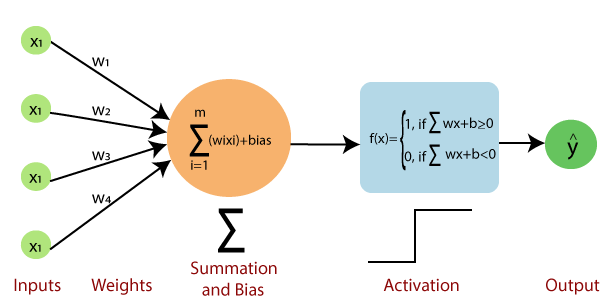
\includegraphics[width = 12cm]{neuron.png}
                  \caption{Replication of how neurons compute the output signal}
                  \label{neuron}
                \end{figure}
 With that intro on neuron/node we will see how a simple neural network looks like as shown figure $\ref{nn}$,
                  \begin{figure}
                   \centering
                   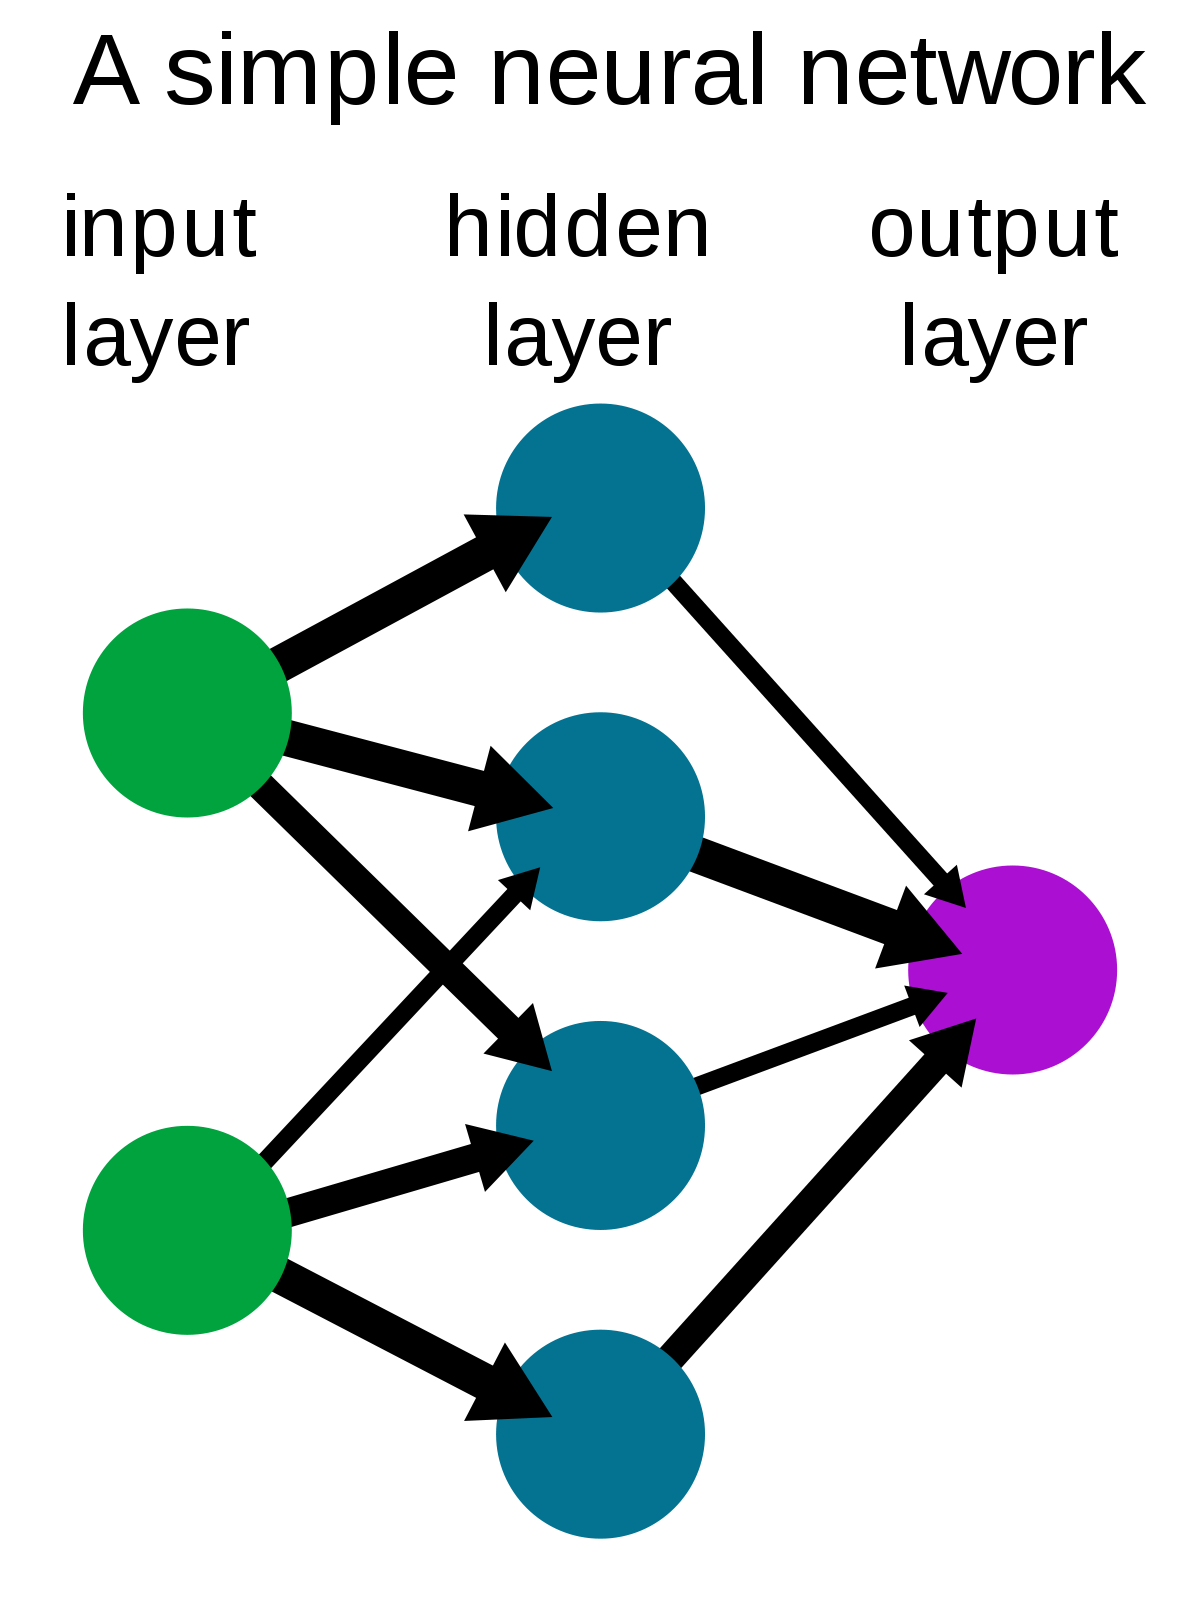
\includegraphics[width=5cm]{neural_network.png}
                   \caption{Simple neural network}
                   \label{nn}
                  \end{figure}
           A simple neural network consists of following things,
              \begin{enumerate}
                 \item \textbf{Input Layer:} Input layer in the neural network comprises of all the information brought by the input neuron. And this information is passed to Hidden layer.
                 \item \textbf{Hidden layer:} The nodes in the hidden layers represents the activation functions and all the computations $\brak{\text{using weights}}$ are done in this layer and passes to the output layer. Note that in general neural network have more than one hidden layers so these computation are continued across these hidden layers using \textbf{weights} and \textbf{bias} until it hits the output layer.
                 \item \textbf{Output Layer:}Here we finally use an activation function that maps to the desired output format.
                 \item \textbf{Connections and weights :} The network consists of Connections b/w the layers which passes the output neuron/node $i$ as the input of  node $j$ along with a weight $W_{j|i}$.And just before surrendering the weighted input to the reciever node , the value will be adjusted with the threshold also known as bias. 
                 \item \textbf{Activation Function :} The activation function defines the output of the node given the input at the node.
                 \item \textbf{Learning Rule:}The learning rule is process of modifying these weights and thresholds $\brak{bias}$ to fit the given input data.
               \end{enumerate}
          So when we find the optimal weights and thresholds of the NN for the input data, we will get the predicted output of the input after travelling all these nodes.
          \section{Types Of Neural Networks}
            \begin{enumerate}
                \item \textbf{ANN} ANN, artificial neural network is basic neural network and the information will flow only in one direction.It is feed-forward neural network.It can also contain hidden layers.It is used for Textual Data or Tabular Data. A widely used real-life application is Facial Recognition. It is comparatively less powerful than CNN and RNN.
                \item \textbf{CNN} Convolutional Neural Network is one of leading flavour of NN at present.It is widely used in Computer vision.
                \item \textbf{RNN} Recurrent Neural Network is better than ANN and less pwerful than CNN.In this type of model, the output from a processing node is fed back into nodes in the same or previous layers. 
            \end{enumerate}
          These neural networks are used in all three types of learning
                 \begin{enumerate}
                   \item Supervised learning
                   \item Unsupervised learning
                   \item Reinforcement learning
                 \end{enumerate}
             \section{Backward Propagation}
       Atlast the optimised weights and bias for the training data are learned using a method known as "Backward Propagation".In this method we will learn the parameters from the output layer i.e., backwards. First we will start by assuming that we know all the weights and bias except the bias before output node and we will intialise this bias with 0 and we will calculate the SSR $\brak{\text{Sum of squares of residuals}}$ and minimise this error using gradient descent method w.r.t the bias.By doing this we will get optimal bias at the output node. From there we go to the intermediate weights and again we will assume that we know all the parameters except these weights and by minimising the SSR we will get optimal weights.It may sound weird but by thinking lot of load will be lift off, this kind of thinking helps in finding optimal weights and bias.
         \end{document}   
